\documentclass{beamer}

% Setup appearance:

\usetheme{Darmstadt}
\usefonttheme[onlylarge]{structurebold}
\setbeamerfont*{frametitle}{size=\normalsize,series=\bfseries}
\setbeamertemplate{navigation symbols}{}


% Standard packages

\usepackage[brazil]{babel}
\usepackage[latin1]{inputenc}
\usepackage{times}
\usepackage[T1]{fontenc}
\usepackage{amsmath}% http://ctan.org/pkg/amsmath
%\usepackage[table]{xcolor}
\usepackage{multicol}
\usepackage{textcomp} 

% Setup TikZ
\usepackage{tikz}
\usetikzlibrary{arrows}
\tikzstyle{block}=[draw opacity=0.7,line width=1.4cm]

%diretório das figuras
\graphicspath{../article}

\title[Nursery]{%
Nursery%
}

\author[Souza,Medeiros,Santos,Ara�jo]{
     Danilo~Souza\and
     Hugo~Santos\and
     Iago~Medeiros\and
     Welton~Ara�jo
     }


\institute[Bel�m]{
  \inst{1}%
  Universidade Federal do Par�
  }
\date[Bel�m 2012]{
  16 de Julho de 2013
  }



\begin{document}
\section{Algoritmo Prisma}
\begin{frame}{Algoritmo}
\begin{itemize}
	\item Para cada classe \textit{c} de 1 a \textit{n}:
	\begin{itemize}
		\item \textbf{Passo 1} - Calcular a probabilidade de ocorr�ncia da classe c para cada par-atributo-valor
		\item \textbf{Passo 2} - Selecionar o pa-atributo com a probabilidade m�xima de ocorr�ncia e crie um subconjunto de treinamento tomado como entrada compreendendo todas as inst�ncias que o par selecionado (para todas as classes)
		\item \textbf{Passo 3} - Repetir os passos 1 e 2 para este subconjunto at� o momento em que ele apresente apenas inst�ncias da classe c. A regra induzida � ent�o a conjun�ao de todos os pares atributo-valor selecionados na cria�ao deste subconjunto homog�neo.
		\item \textbf{Passo 4} - Remover todas as inst�ncias, que satisfa�am a regra formada, do conjunto de treinamento.
	\end{itemize}	
	\item Repetir a sequ�ncia de 1 a  at� que todas as inst�ncias da classe \textit{c} tenham sido removidas.
\end{itemize}
\end{frame}

\begin{frame}{Exemplo - parte I}
\begin{figure}
	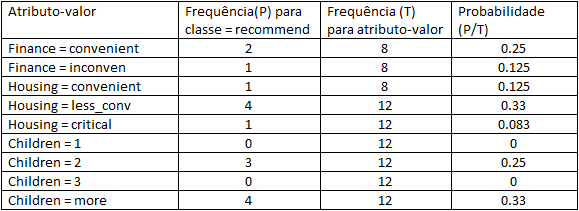
\includegraphics[scale=0.7]{./pictures/prismaTabela1.png}
\end{figure}
\end{frame}

\begin{frame}{Exemplo - parte II}
\begin{figure}
	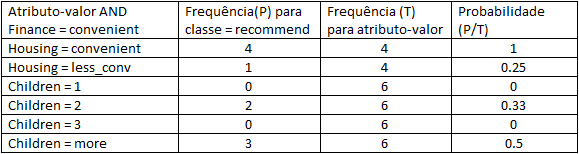
\includegraphics[scale=0.7]{./pictures/prismaTabela2.png}
\end{figure}
\end{frame}

\subsection{Simula��o}
\begin{frame}
	\begin{itemize}
		\item Par�metro variado na simula��o
		\begin{itemize}
			\item Porcentagem da base de dados para treinamento
		\end{itemize}
		\item Par�metros avaliados nas simula��es
		\begin{itemize}
			\item Taxa de erro de classifica��o
			\item Tempo de constru��o do modelo
		\end{itemize}
	\end{itemize}
\end{frame}

\subsection{Resultados}
\begin{frame}{Porcentagem de treinamento}
\begin{figure}
	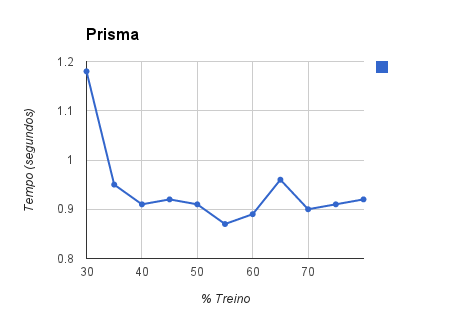
\includegraphics[scale=0.6]{./pictures/PrismaVarTreinoXtempo.png}
\end{figure}
\end{frame}


\begin{frame}{Porcentagem de treinamento}
\begin{figure}
	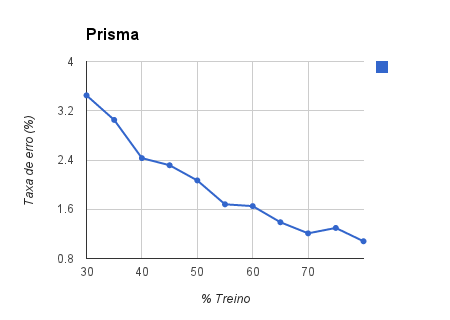
\includegraphics[scale=0.6]{./pictures/PrismaVarTreinoXerro.png}
\end{figure}
\end{frame}


\begin{frame}{Porcentagem de treinamento}
\begin{figure}
	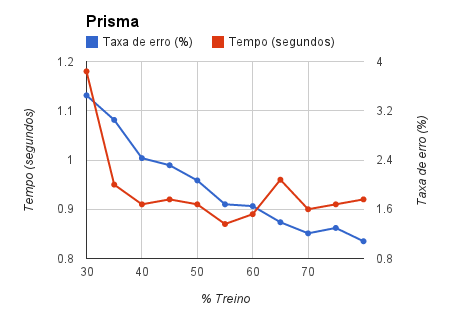
\includegraphics[scale=0.6]{./pictures/PrismaVarTreinoXerro&tempo.png}
\end{figure}
\end{frame}

\end{document}